% !TEX encoding = UTF-8
% !TEX TS-program = pdflatex
% !TEX root = ../arsclassica.tex
% !TEX spellcheck = it-IT

%************************************************
\chapter{Pacchetto RCTBN}
\label{cap:ctbnr}
%************************************************
Uno degli obiettivi di questo lavoro di tesi è consistito nella creazione di un framework in linguaggio \lstinline$R$ per le \acs{CTBN}.

Perciò, in questo capitolo si descrivono i principali aspetti del \pacchettor{}\index{pacchetto \acsfont{R}|see{\acsfont{RCTBN}}}, preposto a tale scopo.

Tuttavia, prima di presentare e chiarire le funzionalità offerte da tale pacchetto, è necessario introdurre il contesto per cui esso è stato pensato, progettato e implementato: il linguaggio \lstinline$R$.

La discussione del presente capitolo segue quindi la logica appena espressa.

Si osservi tuttavia che il corrente capitolo tralascia gli aspetti implementativi del \pacchettor{}, poiché alla loro trattazione e discussione è dedicata l'\vref{cap:guide}.

\section{Il linguaggio R}\label{sec:roverview}
\lstinline$R$\index{\acsfont{R} (linguaggio)} è un linguaggio di programmazione \emph{interpretato} (e al contempo un ambiente di sviluppo) pensato per applicazioni di tipo \emph{statistico}. Esso incorpora di default una vastissima gamma di \emph{funzionalità statistiche} (\eg{} modelli di regressione, test statistici, analisi delle serie temporali, classificazione, clustering) e di tecniche inerenti la \emph{manipolazione dei dati} (\eg{} lazy loading\footnote{Il lazy loading è un design pattern comunemente utilizzato al fine di deferire l'inizializzazione, o il caricamento, di un qualsiasi oggetto finché ciò non sia strettamente necessario.}, strutture dati di tipo tabulare, procedure di calcolo matriciale efficaci) utili allo sviluppo di applicazioni e modelli per l'\emph{analisi dei dati} \citep{R2013}.

\lstinline$R$ supporta principalmente il paradigma di \emph{programmazione funzionale}\index{\acsfont{R} (linguaggio)!programmazione funzionale} con \emph{scoping lessicale}\footnote{Con il termine \emph{scoping lessicale}\index{\acsfont{R} (linguaggio)!scoping lessicale}, o \emph{scoping statico}, ci si riferisce a una determinata modalità di valutazione delle variabili in un dato linguaggio di programmazione. Nello specifico, in un linguaggio con scoping lessicale, il riferimento a un nome di variabile viene risolto basandosi ricorsivamente sulla struttura sintattica che incorpora la definizione di tale nome di variabile. Ne consegue che l'associazione di un valore a una variabile non avviene al momento dell'applicazione e dell'esecuzione bensì durante l'analisi sintattica del sorgente.}. Tuttavia esso può essere esteso al fine di utilizzare il paradigma di \emph{programmazione orientata agli oggetti}.

Lo scoping lessicale, insieme ad altre peculiarità di \lstinline$R$, quali ad esempio il supporto per le \emph{closure}\index{\acsfont{R} (linguaggio)!closure} o le funzioni di prima classe\footnote{Una funzione di prima classe è una funzione che restituisce un'altra funzione. Essa costituisce la più diffusa modalità d'applicazione delle \emph{closure}.}, fanno sì che esso costituisca un ottimo strumento per la creazione di \emph{software scientifico}, così come di applicazioni che richiedono tempi d'esecuzione elevati. In tali casi, infatti, è spesso auspicabile che sia possibile verificare a priori l'eseguibilità o meno del codice sorgente almeno dal punto di vista sintattico \citep{Oliveira2006}.

Una ulteriore caratteristica di \lstinline$R$ è costituita dalla sua natura altamente modulare. Esso è infatti pensato per invogliare l'utilizzatore alla creazione di pacchetti, cioè di porzioni di codice \lstinline$R$ riutilizzabili. A tale scopo \lstinline$R$ fornisce una serie di funzionalità finalizzate alla creazione, pubblicazione e condivisione con la comunità di pacchetti \lstinline$R$. Infatti, tali moduli, una volta sviluppati, possono essere distribuiti in un apposito archivio online di pacchetti \lstinline$R$, chiamato \acs{CRAN}\footnote{Il \acf{CRAN} costituisce la principale fonte di moduli aggiuntivi (\ie{} pacchetti) per \lstinline$R$. Esso è raggiungibile all'indirizzo: \\ \url{http://cran.r-project.org}.}. Questa caratteristica, parallelamente alle precedenti, costituisce una delle principali cause dell'ampia adozione di tale linguaggio di programmazione per l'implementazione di software scientifico.

\subsection{Estendere R}
Poiché lo scopo di questo capitolo è presentare il succitato \pacchettor{}, in questa sottosezione si descrive brevemente il processo di estensione\index{\acsfont{R} (linguaggio)!estensione} di \lstinline$R$, attuabile, come detto, tramite la creazione di moduli chiamati pacchetti.

Un pacchetto \lstinline$R$ consiste in un insieme di cartelle e file che rispettano determinate convenzioni. Nello specifico, data una cartella radice che si intende utilizzare come contenitore del sorgente di un qualsiasi pacchetto \lstinline$R$, è necessario che essa contenga almeno i seguenti elementi:
\begin{itemize}
	\item una sotto cartella \lstinline$R/$, in cui è necessario inserire i sorgenti in linguaggio \lstinline$R$ del pacchetto
	\item un file \lstinline$DESCRIPTION$, che descriva il pacchetto, il suo scopo, le sue dipendenze da altri pacchetti, la licenza con cui viene distribuito e l'autore.
\end{itemize}
La struttura di un pacchetto \lstinline$R$ prevede ulteriori elementi opzionali:
\begin{itemize}
	\item una sotto cartella \lstinline$man/$ preposta alla documentazione del pacchetto
	\item un file \lstinline$NEWS$ per la descrizione dei cambiamenti in ogni versione del pacchetto tramite il formato standard che \lstinline$R$ fornisce a tale scopo
	\item un file \lstinline$README$ che contenga una panoramica generale del pacchetto
	\item un file \lstinline$inst/CITATION$ finalizzato alla descrizione delle modalità con cui citare il corrente pacchetto in lavori scientifici
	\item una sotto cartella \lstinline$demo/$ contenente delle applicazioni d'esempio che utilizzano il pacchetto stesso
	\item una sotto cartella \lstinline$inst/doc$ contenente la documentazione approfondita e eventuali manuali d'utilizzo
	\item un file \lstinline$NAMESPACE$ che descriva quali funzioni devono far parte della \acs{API} del pacchetto cosicché esse siano utilizzabili dagli utenti
	\item le sotto cartelle \lstinline$test/$ e \lstinline$inst/test/$ contenenti i test per il pacchetto, allo scopo di assicurarsi che esso operi come progettato
	\item una sotto cartella \lstinline$data/$ preposta all'incorporazione nel pacchetto di eventuali dataset d'esempio
	\item una sotto cartella \lstinline$src/$ per il codice sorgente non in linguaggio \lstinline$R$ (\eg{} \CC{}, \lstinline$C$ o \lstinline$FORTRAN$)
	\item una sotto cartella \lstinline$exec/$ preposta alla distribuzione di ulteriori script eseguibili
	\item una sotto cartella \lstinline$po/$ che contenga i file di traduzione per il pacchetto.
\end{itemize}
\`E possibile creare la struttura di un pacchetto \lstinline$R$ manualmente o usufruendo della funzione base \lstinline[language=rstats]{package.skeleton}. Inoltre, a titolo informativo, si evidenza l'esistenza di un pacchetto esterno finalizzato alla facilitazione di tale processo, il pacchetto \lstinline[]|devtools| \citep{DEVTOOLS2013} (si veda l'\vref{cap:guide} per maggiori dettagli a riguardo).

Infine, si fornisce una panoramica delle pratiche consigliate (o necessarie) riguardanti gli elementi obbligatori per la creazione di un pacchetto \lstinline$R$.

La sotto cartella \lstinline$R/$ non impone alcun vincolo sull'organizzazione del codice sorgente che essa deve contenere, aldilà del fatto che esso deve essere codice in linguaggio \lstinline$R$. Tuttavia, quando si intende sviluppare utilizzando l'approccio funzionale, venendo meno, almeno esplicitamente, il concetto di classe, è pratica consolidata e consigliata organizzare il codice sorgente in diversi file in base all'area tematica cui appartengono le funzioni che essi contengono.

Invece, il file \lstinline$DESCRIPTION$, al fine di definire i metadati del pacchetto \lstinline$R$, deve contenere determinati campi.

Il sorgente \ref{lst:rpackex} illustra, tramite un esempio di file \lstinline$DESCRIPTION$ per \rctbn{}, tale pratica.
\vspace*{8pt}\inputsourcecode[numbers=none,caption={[File di descrizione di un pacchetto \lstinline$R$]Esempio di possibile file di descrizione del \pacchettor{}.},language=pseudo,label=lst:rpackex]{codes/samplerpackage}\vspace*{8pt}
Di seguito si elencano i sei campi che tale file di testo deve obbligatoriamente contenere:
\begin{itemize}
	\item il campo \lstinline$Package$ che definisce il nome del pacchetto (e dovrebbe, in teoria, corrispondere al nome della cartella radice)
	\item il campo \lstinline$Title$ contenente una descrizione sintetica del pacchetto (massimo una linea di testo)
	\item il campo \lstinline$Description$ preposto a una descrizione maggiormente dettagliata del pacchetto e delle sue funzionalità
	\item il campo \lstinline$Version$ contenente il numero di versione, auspicabilmente nel formato \lstinline$major.minor.patchlevel$
	\item il campo \lstinline$Mantainer$ contenente un singolo nome e indirizzo e-mail per la persona responsabile della manutenzione del pacchetto
	\item il campo \lstinline$License$ contenente una abbreviazione standard di una licenza open source.
\end{itemize}

\section{Analisi}\label{sec:rctbn-describ}
In questa sezione si descrive per grandi linee il \pacchettor{}\index{\acsfont{RCTBN}}.

Lo scopo di tale pacchetto, come detto, consiste nell'implementazione del framework delle \acs{CTBN}: esso espone perciò una collezione di funzioni (\ie{} \acs{API}) correlate ai modelli \acs{CTBN} e \acs{CTBNC}.

Al fine di presentare le funzionalità di tale pacchetto, di seguito, si riportano i requisiti cui esso aderisce.
\begin{description}
	\item[R1 -- Gestione dei dataset] \hfill \\
	Il pacchetto deve permettere di caricare nel minore tempo possibile insiemi di dati completi (eventualmente di dimensioni considerevoli) presenti sul disco rigido dell'utente. Il sistema deve fornire all'utente un'interfaccia che semplifichi questo processo nascondendo e automatizzando la scelta dei percorsi di ricerca e memorizzazione dei dataset.
		\begin{description}
		\item[R1.1 -- Importazione] \hfill \\
		Il pacchetto deve consentire di importare insiemi di \emph{dati completi}. Gli insiemi di dati corrispondono a insiemi di file posti nella medesima cartella. Tali file possono essere in qualsiasi formato testuale (\eg{} \acs{CSV}, \acsfont{TSV}, \acsfont{TXT}) purché essi contengano una struttura tabulare, specificabile dall'utente. Il sistema in esame deve controllare che determinati vincoli, propri del modello in questione, siano rispettati cosicché ogni dataset importato possa realmente rispecchiare un modello \acs{CTBN}. Si elencano i controlli necessari:
		\begin{itemize}
			\item controllare che ogni file contenga i dati relativi all'evoluzione temporale (\ie{} colonna temporale)
			\item controllare che ogni file contenga una colonna classe e che il suo valore sia univoco per ogni file, nel caso l'utente lo richieda
			\item controllare che ogni file contenga delle traiettorie di dati completi.
		\end{itemize}
		\item[R1.2 -- Serializzazione] \hfill \\
		Il sistema deve consentire all'utente di comprimere e serializzare il dataset importato, in modo automatico o manuale, su disco rigido.
		\item[R1.2 -- Caricamento veloce] \hfill \\
		Il sistema deve permettere, in qualsiasi momento, il caricamento veloce di un qualsiasi dataset precedentemente importato e serializzato.
		\end{description}
		Si osservi che tali processi devono poter essere eseguiti anche in sessioni di lavoro diverse.
	\item[R2 -- Apprendimento di un modello CTBN] \hfill \\
	Il pacchetto deve consentire l'apprendimento dei parametri di un modello \acs{CTBN} rispetto a un insieme di dati completi precedentemente importato e processato. La natura del modello (\ie{} la struttura del grafo) che l'utente intende apprendere deve essere specificata ad ogni esecuzione.
		\begin{description}
		\item[R2.1 -- Computazione statistiche sufficienti] \hfill \\
		Il sistema deve permettere il calcolo delle \emph{statistiche sufficienti} consentendo all'utente di selezionare l'insieme di nodi (e i rispettivi insiemi di genitori) da sottoporre a tale processo, come mostrato nella \autoref{subsec:ctbn-sufficient-stats} \vpageref{subsec:ctbn-sufficient-stats}.
		\item[R2.2 -- Computazione iper-parametri] \hfill \\
		Il sistema deve consentire il calcolo degli \emph{iper-parametri} di un modello \acs{CTBN} a partire da delle statistiche sufficienti precedentemente calcolate, come mostrato nella \autoref{subsec:ctbn-params} \vpageref{subsec:ctbn-params}.
		\item[R2.3 -- Computazione matrici di intensità condizionali] \hfill \\
		Il pacchetto deve permettere il calcolo delle \emph{\im{}} a partire dagli iper-parametri.
		\end{description}
	\item[R3 -- Apprendimento strutturale di un CTBN] \hfill \\
	Il pacchetto deve consentire l'apprendimento della struttura di un modello \acs{CTBN} dato un insieme di dati completo. L'utente deve poter specificare, qualora lo desideri, l'approccio da utilizzare (attualmente si fornisce solo un approccio basato su punteggio, quello descritto nel \vref{cap:structurallearning}).
		\begin{description}
			\item[R3.1 -- Ricerca euristica] \hfill \\
			Il sistema deve fornire un modulo preposto alla ricerca euristica della struttura \acs{CTBN} ottimale. Attualmente è prevista solamente la procedura di ricerca \emph{\hc{}} con memoizzazione\footnote{La \emph{memoizzazione} è una tecnica di ottimizzazione delle chiamate delle funzioni finalizzata al miglioramento dei tempi d'esecuzione di un sistema software e al risparmio di risorse computazionali. Essa consiste nel salvare in memoria il risultato ottenuto dalla chiamata di una funzione, comprensiva di parametri attuali, in modo da non dover effettuare nuovamente la computazione in caso la funzione in questione venga nuovamente chiamata con gli stessi parametri attuali. Nel contesto dell'apprendimento strutturale di una \acs{CTBN} questa tecnica può essere usata con efficacia evitando di computare nuovamente il punteggio di un modello \acs{CTBN} già processato precedentemente.} (a tal riguardo si rimanda alla \autoref{subsec:structurallearning-hc} \vpageref{subsec:structurallearning-hc}).
			\item[R3.2 -- Funzione di punteggio] \hfill \\
			Il sistema deve fornire una funzione di punteggio delle strutture \acs{CTBN} (attualmente è prevista solamente la computazione dello \emph{score bayesiano}, presentata nella \vref{sec:ctbn-structurallearning-score}).
		\end{description}
	\item[R4 -- Classificazione tramite modelli CTBNC] \hfill \\
	Il pacchetto deve permettere, tramite l'utilizzo di un classificatore \acs{CTBNC}, la \emph{classificazione supervisionata} di traiettorie multi-variate che evolvono nel tempo continuo. L'utente deve immettere nel sistema l'istanza per cui inferire la classe di appartenenza e selezionare il classificatore da utilizzare per classificarla.
		\begin{description}
		\item[R4.1 -- Apprendimento di un classificatore CTBN] \hfill \\
		Tale processo incorpora quello relativo al punto {\bfseries\spacedlowsmallcaps{R2}}. In aggiunta, esso deve computare la probabilità a priori della variabile classe sull'insieme di dati completi di input. Il pacchetto deve fornire sia una versione generale del processo di apprendimento, funzionante per qualsiasi classificatore \acs{CTBN} (\ie{} \autoref{lst:ctbnc-learning} presentato a \vpageref{lst:ctbnc-learning}), sia una versione dedicata esclusivamente ai classificatori \acs{CTNB} (\ie{} \autoref{lst:ctnbc-learning} presentato a \vpageref{lst:ctnbc-learning}).
		\item[R4.2 -- Inferenza tramite classificatore CTBN] \hfill \\
		Il sistema deve consentire all'utente, dato un qualsiasi classificatore \acs{CTBN}, di classificare una qualsiasi istanza completa dei dati assegnando ad essa la classe che ottiene il valore maggiore di probabilità secondo l'\autoref{lst:ctbnc-inference} presentato a \vpageref{lst:ctbnc-inference}.
		\end{description}
\end{description}
Si osservi che è stata tralasciata la discussione di una serie di ulteriori requisiti e relative funzionalità, quali ad esempio quelle relative all'esecuzione della \emph{cross-validazione} e al calcolo delle \emph{metriche di valutazione} dei classificatori, poiché esse riguardano direttamente l'argomento primario di questo lavoro di tesi e, inoltre, sono state implementate separatamente come pacchetti \lstinline$R$ indipendenti da \rctbn{}.

La principale entità che tale pacchetto rappresenta corrisponde al modello \acs{CTBN}. Tale entità è composta dal grafo ad essa sottostante e dall'insieme dei parametri e eventualmente delle \im{} relative ad ogni nodo di tale grafo, secondo la \autoref{defn:ctbn} a pagina \pageref{defn:ctbn}.

Parimenti, \rctbn{} può rappresentare anche i modelli \acs{CTBNC}, che costituiscono, come specificato dalla \autoref{defn:ctbnc} a pagina \pageref{defn:ctbnc}, una specializzazione del modello \acs{CTBN}. Il vincolo che tale specializzazione apporta corrisponde all'esistenza di un particolare nodo radice: il nodo classe.

Si noti infine che ognuna delle succitate macro funzionalità corrisponde a un componente del \pacchettor{} e viene implementata separatamente dalle altre.

Quindi, al fine di chiarire ulteriormente l'architettura del \pacchettor{} e le relazioni che intercorrono tra i componenti da cui esso è costituito, la \vref{fig:rctbncomponents} ne illustra il relativo diagramma dei componenti.
\begin{figure}[ht]
	\centering
	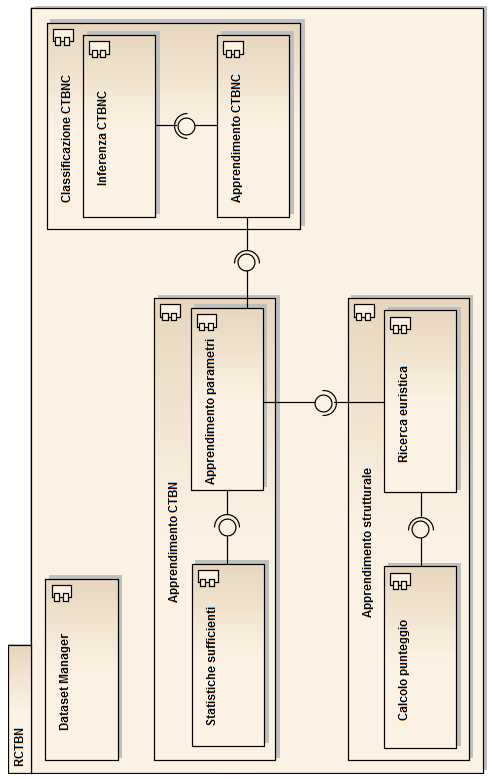
\includegraphics[width=1.1\columnwidth,center]{rctbn-arch.png}
	\caption[Diagramma dei componenti di \rctbn{}]{Diagramma dei componenti di \rctbn{}.}
	\label{fig:rctbncomponents}
\end{figure}
Tale diagramma evidenzia le interfacce di comunicazione fra i vari componenti e la loro corrispondenza rispetto alle funzionalità descritte precedentemente.
